\documentclass[12pt]{jreport}
\usepackage{comment}
\usepackage{./sty/eclepsf}
\usepackage{tascmac}
\usepackage{tabularx}
\usepackage{listliketab}
\usepackage[longnamesfirst]{natbib}
\usepackage[dvipdfmx]{graphics}
\usepackage[dvipdfmx]{graphicx}
\usepackage[dvipdfmx]{color}
\usepackage{subfigure}
\usepackage{alltt}
\usepackage{here}
\usepackage{afterpage}
\usepackage{./sty/ncodeline}
%\usepackage[dvipdfmx, colorlinks, breaklinks,%
\usepackage[dvipdfmx, breaklinks,%
bookmarks=true, bookmarksnumbered=true,%
bookmarkstype=toc, bookmarksopen=true,bookmarksopenlevel=3,%
pdftitle={RG},%
]{hyperref}
\usepackage{bookmark}
\usepackage{lscape}

\AtBeginDvi{\special{pdf:tounicode EUC-UCS2}}

\usepackage{fancyhdr}

\usepackage{./sty/doxygenorig}

\usepackage{indentfirst}
\usepackage{url}
\usepackage{listings,./sty/jlisting}

\def\lstlistingname{プログラム}

\lstset{%
 language={C++},
 %backgroundcolor={\color[gray]{.85}},%
 basicstyle={\small\ttfamily},%
 identifierstyle={\small},%
 commentstyle={\small\itshape},%
 keywordstyle={\small\bfseries},%
 ndkeywordstyle={\small\ttfamily},%
 stringstyle={\small\ttfamily},
 frame={tb},
 framesep=1zw,
 breaklines=true,
 numbers=left,%
 xrightmargin=0zw,%
 xleftmargin=1.5zw,%
 numberstyle={\scriptsize},%
 stepnumber=1,
 numbersep=1zw,%
 lineskip=-0.5ex%
}

\usepackage{amssymb}
%\usepackage{supertabular,multirow}

\usepackage{array}
\newcolumntype{M}[1]{>{\centering\arraybackslash}m{#1}}

% A4  size: 297mm*210mm %1pt = 0.35mm
\setlength{\topmargin}{-3.4mm} % 10pt 25.4mm - 3.4mm = 22mm
\setlength{\oddsidemargin}{-0.4mm} % 25.4mm - 0.4mm = 25mm
\setlength{\evensidemargin}{-0.4mm} % 25.4mm - 0.4mm = 25mm
\setlength{\textheight}{231mm} % 660pt % original is 225.75mm 645pt
\setlength{\textwidth}{160mm} % 457pt

\renewcommand{\topfraction}{.99}
\renewcommand{\textfraction}{.0}
\renewcommand{\floatpagefraction}{.99}
\renewcommand{\bibname}{参考文献}


\pagestyle{fancy}
\lhead[]{}

\makeatletter
\def\chaptermark#1{\markboth {\ifnum \c@secnumdepth>\m@ne
\@chapapp\ \thechapter \@chappos\ \fi #1}{}}
\makeatother

% タイトル
\def\title{惑星規模の分散システムのための試験環境の設計と構築}
% 英語タイトル
\def\etitle{Designing and Implementation the test environment for planetary-scale distributed system}
% 著者(日本語)
\def\author{廣川昂紀}
% 著者(英語)
\def\eauthor{Koki Hirokawa}
% 学部・研究科
\def\dept{慶應義塾大学 環境情報学部}
% 学部・研究科(英語)
\def\edept{Keio University Faculty of Environment and Information Studies}

\begin{document}

\pagenumbering{roman}
\begin{titlepage}
  \begin{center}
    \begin{large}
      卒業論文 2019年度(令和元年)\\
      \vspace{24pt}
      \title
      \end{large}
  \end{center}
  \vspace{40em}
  \begin{flushright}
    \large \dept\\
    \author
  \end{flushright}
\end{titlepage}

\thispagestyle{empty}


卒業論文要旨 - 2019年度 (令和元年度)
\begin{center}
\begin{large}
\begin{tabular}{|M{0.97\linewidth}|}
    \hline
      \title \\
    \hline
\end{tabular}
\end{large}
\end{center}

~ \\
本研究では、地理的分散システムの検証実験におけるコミュニケーションコストとヒューマンリソースのオーバーヘッドを解決するための
システムを提案する。
ブロックチェーンの基盤技術として知られるP2Pネットワークなどは、地理的に分散したノードによって形成されており、これらは従来の
クライアント・サーバ方式のソフトウェアに比べテストが行いづらい。
何故なら、実際に離れた地点に設置されたノードを用いてテスト用のステージング環境を構築するためには、多くの人手とその間での
コミュニケーションが必要になるからである。

そこで、OpenVPNとKubernetesを利用することで地理的かつネットワーク上で論理的に離れたノードを統合管理できるステージング環境
を構築する。特定のポイントから一斉にすべてのノードに対しての操作を行うことで、デプロイ作業やアップデート作業における
コミュニケーションコストとヒューマンリソースを解決することが可能だと考えた。

本システムの実装後、実際にネットワーク上で別セグメントに点在するノードに対して特定のポイントから一斉にソフトウェアを起動、
更新、停止できることを確認して、本研究での提案が実現可能であることを証明する。

評価として、BSafe.networkにて本システムを使用しなかった場合と使用した場合で、作業工程数にどれほどの差が生じるかを検証した。
結果、本システムを使用した場合には大きく工程数を削減することができ、本研究で課題とした地理的分散システムの検証実験における
コミュニケーションコストとヒューマンリソースのオーバーヘッドを解消可能にした。

よって本研究は、地理的分散システムの開発における検証作業の効率性を促進し、システムの堅牢性の向上に役立つと考える。
~ \\
キーワード:\\
\underline{1. 地理的分散システム},
\underline{2. ステージング環境},
\underline{3. OpenVPN},
\underline{4. Kubernetes}
\begin{flushright}
\dept \\
\author
\end{flushright}

\thispagestyle{plain}
\clearpage

Abstract of Bachelor's Thesis - Academic Year 2019
\begin{center}
\begin{large}
\begin{tabular}{|p{0.97\linewidth}|}
    \hline
      \etitle \\
    \hline
\end{tabular}
\end{large}
\end{center}

~ \\
In this study, we propose a system design for a experiment environment of a planetary-scale distributed system.
The planetary-scale distributed system in this study is a distributed system consisted of geographically distributed computers.
P2P is one of the technologies for planetary-scale distributed systems.
P2P system does not require a centralized server and is run by computers that have an equal relationship with each other to cooperate.
Blockchain is one of the P2P systems.
The experiment for planetary-scale distributed systems should consider network latency.
Therefore, the experiment environment for planetary-scale distributed systems should consist of geographically distributed servers.

There are the PlanetLab and the cloud services, the BSafe.network as the experiment environment for planetary-scale distributed systems, but these have problems.
PlanetLab is a research network that supports the development of network services.
It has 1353 servers that are able to be controlled via ssh in 717 areas around the world but can not flexibly change an environment of the server such as OS, CPU, and memory.
In a public cloud service, servers can be geographically distributed by specifying an area of a data center called region.
However, regions are limited and network performance is high around a data center of a public cloud service and the delay in network communication is less than the public production environment.
BSafe.network is the network for researching the blockchain technology that consists of 32 universities around the world.
In the BSafe.network, developers can research using servers owned by each university.
However, the manual operation of each operator is needed for the joint research between universities, because the management authority of each server is divided.
To solve these problems, we propose the system design for the integrated experiment environment by combining OpenVPN and Kubernetes.
In this system, it is possible to run experiments with the delay in network communication, regardless of where the servers are geographically distributed.
In addition, multiple applications can be run on a single server in various environments by utilizing virtualization technology, and
can integrate even when each server is under separate management.

We verified whether integrated management of all servers is possible and whether this system operates normally considering the delay in communication.

This research makes it possible to run experiments for planetary-scale distributed systems more flexibly in a similar manner to a public production environment.
Even if each server is under separate management such as BSafe.network,
It is possible to implement an integrated experiment environment without any manual works.

~ \\
Keywords : \\
\underline{1. Geographically Distributed System},
\underline{2. Staging Environment},
\underline{3. OpenVPN},
\underline{4. Kubernetes}
\begin{flushright}
\edept \\
\eauthor
\end{flushright}

\thispagestyle{plain}
\clearpage

\tableofcontents\thispagestyle{plain} %目次
\clearpage
\listoffigures\thispagestyle{plain} %図目次
\clearpage
\listoftables\thispagestyle{plain} %表目次
\clearpage

\pagenumbering{arabic}
\chapter{序論}
\label{introduction}

本研究では,惑星規模の分散システムのための試験環境の設計と構築を行う.

本章では,惑星規模の分散システムを定義し,本研究の背景である惑星規模の分散システムの発達とシステムの試験環境について概説する.
本研究の課題を明らかにした上で,目的を明確化し,目的を達するための仮説を示す.
最後に仮説を裏付けるための提案手法を示し,本研究の概要を示す.

\section{本研究の背景}
\label{introduction:background}

本節では,本研究の背景について述べる.

初めに,本研究が対象とする惑星規模の分散システムと試験環境について概説する.
分散システムについて概説した上で惑星規模の分散システムを定義し,惑星規模の分散システムの発達について述べる.
加えて,惑星規模の分散システムに求められる試験環境について説明する.

\subsection{惑星規模の分散システム}

本節では,本研究における惑星規模の分散システムを定義する.

分散システムは,複数の構成要素が組み合わさって動作するシステムである.
各構成要素は独立しており,互いに協調動作することによってシステム全体が成り立っている.

惑星規模の分散システムは,分散システムの中でも世界中に地理的に分散したコンピュータによって構成されるものを指す.
惑星規模の分散システムの基盤技術としては,P2Pがあげられる.

P2Pは``Peer to Peer''の略記であり,中央集権的なサーバを必要とせず,各コンピュータが互いに対等な関係を築き協調動作することで成り立つシステムモデルまたはその技術自体を指す.
P2Pは,システム内に明確な役割分担と主従関係のあるクライアントサーバモデルとは対照的なシステムモデルである.
クライアントサーバモデルは中央主権的なシステムであり,通信において常にクライアントとサーバで一対一の関係が成り立つ.
クライアントはサーバに対し処理や情報を要求し,要求を受け取ったサーバは特定の処理を行なってクライアントへ返答する.
対してP2Pシステムでは,システムを構成する各コンピュータの役割は状況に応じて柔軟に変化し,通信において多対多の関係が成り立つ.
クライアントとして他のコンピュータに対し要求する場合もあれば,他のコンピュータからの要求に対して応答する場合もある.
クライアントサーバモデルに比べて,拡張性(スケーラビリティ)ならびに耐障害性において優れているのが特徴的である.

ビットコインの中核技術であるブロックチェーンは,P2Pシステムの一例である.
ブロックチェーンのようなP2Pシステムでは,地理的に分散することによるネットワークでの通信の遅延を考慮した上で協調動作可能であることを開発者は意識しなければならない.

\subsection{惑星規模の分散システムの発達}

2000年代初頭,Winny~\cite{Winny}やGnutella~\cite{Gnutella}といった惑星規模の分散システムが頭角を現した.
どちらのサービスもP2P技術を基盤としており,それまでシステムモデルとして一般的であったクライアントサーバモデルとは異なる形態を採用したことで注目が集まった.
P2P技術が研究分野で取り上げられる頻度も多くなり,サービスとしても今後一層幅を広げていくと思われたが,クライアントサーバモデルに置き換わるまでの隆盛はなく後退していった.
しかし,2008年にSatoshi NakamotoによりBitcoinのために開発されたブロックチェーン技術が登場することによって,再度P2P技術が脚光を浴びるようになり,開発や研究の勢いが再び盛んになってきている.

\subsection{試験環境}

試験環境とは,公の実稼働環境での運用をする前にシステム全体の試験を行うための環境である.
開発者が実際に開発を行う開発環境と公の実稼働環境では,環境の差異から動作の違いが生じ,開発環境で正常に動作していたものが公の実稼働環境に反映した途端動作しなくなるといった事象が度々発生する.
そのような事態を防ぐために開発環境と公の実稼働環境の間に試験環境を構築し,公の実稼働環境への適用前に試験環境にてシステム全体の試験をすることで予想外の障害が発生する可能性を低減できる.
惑星規模の分散システムにおいても,システムの不具合を早期に発見するために試験環境が必要である.

先に述べたように,惑星規模の分散システムでは地理的に分散することによるネットワークでの通信の遅延が発生する.
よってシステムの試験は,通信の遅延を考慮した上で正常に協調動作することを確認する必要があるため,試験環境は地理的に分散したサーバによって構成されたものでなければならない.

既存の惑星規模の分散システムの試験環境としては, PlanetLabやクラウドサービスの活用, BSafe.networkがあげられる.
PlanetLabは,ネットワークサービスの開発を支援する研究ネットワークであり,世界中の717地域1353のサーバを利用することができ,
クラウドサービスでは,リージョンと呼ばれるデータセンターの地域を指定することでサーバを分散配置することが可能である.
最後に,BSafe.networkは32の大学によって構成されるブロックチェーン技術の研究を行うためのネットワークであり,世界中の各大学が保有するサーバを用いて開発を行える.

\begin{figure}[htbp]
  \begin{center}
    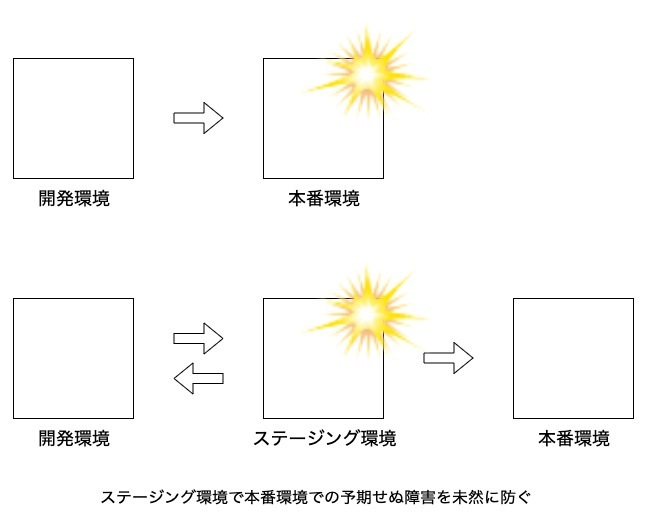
\includegraphics[width=0.8\textwidth]{./figures/staging.jpg}
    \caption{試験環境}
  \end{center}
\end{figure}

\section{本研究の課題と目的}
\label{introduction:issue-aim}

本節では,本研究の課題と目的を述べる.

まず,~\ref{introduction:background}章で述べた本研究の背景を元に,惑星規模の分散システムの試験環境における課題を示す.
その上で本研究の目的を明確にする.

\subsection{本研究の課題}
\label{introduction:issue-aim:issue}

本研究では,既存の惑星規模の分散システムの試験環境の課題について指摘する.

惑星規模の分散システムの試験では,地理的に分散配置されることによるネットワークでの通信の遅延を考慮した上で各コンピュータが正常に協調動作を行えるかを確認する必要があり,
試験環境では各サーバを実際に地理的に分散配置する必要性があることは~\ref{introduction:background}章の背景で述べた通りである.
さらに既存の試験環境として, Planet Labやクラウドサービスのリージョンの活用, Bsafe.networkがあげられるが,それぞれ課題があると考える.
Planet Labでは世界中に分散したサーバを利用することが可能だが, OSやCPU,メモリなどのサーバの環境を柔軟に変更することができない.
クラウドサービスでは,サーバの環境を自由に変更可能であり,リージョンを活用して地理的に分散した場所にサーバを設置することができるが,
リージョンが限定的であり,公の実稼働環境に比べネットワークでの通信の遅延が少ないため,環境に差異が生じてしまう.
BSafe.networkでは,世界中の32の大学が保有するサーバを用いてシステムの試験を行えるが,各サーバの管理権限が各大学のオペレータに委ねれられているため,
大学間での共同研究を行う場合にオペレータの手作業が介入してしまう.

本研究では,このように惑星規模の分散システムの試験環境の構築手法が整備されていないことを課題とする.

\subsection{本研究の目的}
\label{introduction:issue-aim:aim}

本研究では,惑星規模の分散システムのための試験環境の構築手法を提案することを目的とする.

\section{本研究の仮説}
\label{introduction:hypothesis}

~\ref{introduction:issue-aim:issue}章で述べた課題を解決するため,本研究では地理的に分散したサーバを統合管理可能な試験環境の構築が必要であると考えた.
惑星規模の分散システムの試験環境は,
\begin{itemize}
  \item OSやCPU, Memoryといったサーバ環境を柔軟に変更可能であること
  \item 公の実稼働環境を想定したネットワークでの通信の遅延を考慮できること
  \item 異なる管理権限下にある各サーバに対し統合的管理が可能であり,各オペレータの手作業を低減できること
  \item 地理的に分散した各サーバに対し,統合的な操作が可能であること
\end{itemize}
の四点を満たさなければならない.

本研究では,上記の必要要件を満たすことで~\ref{introduction:issue-aim:issue}で述べた課題点を解決し,
~\ref{introduction:issue-aim:aim}で述べた惑星規模の分散システムの試験環境の構築手法の提案を達成できると考えた.

\section{本研究の手法}
\label{introduction:proposal}

本研究では,~\ref{introduction:hypothesis}章で述べた必要要件を満たすため,OpenVPNとKubernetesを組み合わせた惑星規模の分散システムの統合的試験環境を提案する.

Kubernetesはコンテナオーケストレーションツールであり,コンテナ化仮想技術によってコンテナ化されたアプリケーションのデプロイやスケーリングを自動化し,統合管理するためのシステムである.
Kubernetesでは複数のサーバでクラスタを構成しており,クラスタリングを行うためには各サーバが互いにIPレベルで疎通可能な状態になければならない.
よって,IPレベルでの疎通が取れない別々のセグメントに配置されたサーバ間ではKubernetesクラスタを構築することはできない.

そこで地理的に分散し異なるセグメントに配置されたサーバ間を繋ぐOpenVPNオーバーレイネットワークを構築することで,各サーバを互いにIPレベルで疎通可能にする.
OpenVPNは,VPNネットワークの構築をソフトウェアで実現するために開発されたオープンソースソフトウェアである.

本研究では, OpenVPNとKubernetesを組み合わせ,地理的に分散した拠点間で形成したOpenVPNオーバーレイネットワーク上でKubernetesクラスタを構築した.
本システムが本研究における課題点を解決できているか推定することで,要件を満たせることを確認した.

\section{本論文の構成}
\label{introduction:structure}

本論文における以降の構成は次の通りである.

~\ref{background}章では,惑星規模の分散システムと試験環境ならびに本研究で使用する技術について概説し,本研究の背景を明確化する.
~\ref{issue}章では,本研究における課題を明確化し,課題を解決するための要件,仮説と手法について概説する.
~\ref{implementation}章では,本研究で提案する試験環境の構築方法について述べる.
~\ref{evaluation}章では,\ref{issue}章で述べた課題に対しての評価を行い,考察する.
~\ref{conclusion}章では,本研究のまとめと今後の課題についてまとめる.

%%% Local Variables:
%%% mode: japanese-latex
%%% TeX-master: "../thesis"
%%% End:

\chapter{背景}
\label{background}

本章では本研究の背景と関連する技術について概説する.

\section{惑星規模の分散システム}
\label{bg:definition}

本節では、本研究が対象とする惑星規模の分散システムの定義を明らかにする。
定義を分かりやすくするため、先にモノリスと分散システムについて概説し、違いを明らかにした上で惑星規模の分散システムを定義する。

\subsection{モノリス}
\label{bg:definition:monolith}

モノリスとは、モノシリックなシステムを指す。
モノリスは英語で一枚岩を意味し、システムにおいては、大きな単一のプログラムによって特定の処理を実行するアーキテクチャといえる。
このように、本来では大量のコードによって成り立つという意味を含むが、比較化のため本研究では、プログラムの大きさに関わらず単一のコンポーネントで構成されたシステムをモノリスと呼ぶことにした。
単一のコンポーネントで構成されるシステムはアーキテクチャがシンプルなため、システム自体が小さい場合は取り扱いやすい。
しかし、システムが大きくなるにつれて機能同士の依存関係が密な状態になることで細かい粒度でテストを行えなかったり、チーム開発における並行作業が困難になる傾向にある。

\subsection{分散システム}
\label{bg:definition:distributed-system}

分散システムとは、マイクロサービスアーキテクチャなシステムを指す。
システム全体が複数の独立したコンポーネントを組み合わせて成り立っている点において、モノリスとは対照的である。
各コンポーネントは異なる役割を持っており、お互いに協調動作することによってシステム全体が動作する。
本研究で使用するKubernetesも、コンテナオーケストレーションに必要な機能をコンポーネント毎に分割した分散システムである。
Kubernetesに関する説明は~\ref{background:container-orchestration-system:kubernetes}章で詳しく行う。
分散システムは複雑で取り扱いづらいように思われるが、実際には機能が細分化され各コンポーネントの役割が明確になる。
機能同士の依存関係が希薄になるため細かい粒度でのテストが可能となり、障害時の原因特定も容易になる。
チーム開発において開発者同士で同じ箇所を担当する可能性も下がるため、開発スピードが向上するというメリットもある。

\subsection{惑星規模の分散システム}
\label{bg:definition:planetary-scale-distributed-system}

本研究で対象とする惑星規模の分散システムとは、~\ref{definition:distributed-system}の中でも世界中に地理的に分散したコンピュータが協調動作することによって成り立つシステムを指す。
近年注目を集めているブロックチェーンや2000年代初頭に登場したWinnyといったサービスが、惑星規模の分散システムにあたる。
これらのシステムに使用されている技術や、サービスについての概説は~\ref{bg:planetary-scale-distributed-system}にて行う。
惑星規模の分散システムは、システムを構成するコンピュータの場所を開発者が固定できないことと、システム全体がスケーリングしていく点で~\ref{bg:definition:distributed-system}章の分散システムとは異なる。
開発者は、コンピュータの位置やスケーリングした際の挙動を考慮した上で開発を行わなければならない。
よって、システムの挙動を左右する条件が~\ref{bg:definition:monolith}章のモノリスや~\ref{bg:definition:distributed-system}章の分散システムに比べて多くテストが難しい。

\section{惑星規模の分散システムにおける使用技術と参考例}
\label{bg:planetary-scale-distributed-system}

本節では、~\ref{bg:definition:planetary-scale-distributed-system}章で概説した惑星規模の分散システムの主な使用技術とサービスの参考例について概説する。
使用技術としては、P2Pが一番にあげられる。
クライアントサーバモデルとは異なるシステムモデルであり、最近ではブロックチェーン技術にも取り入れられている。
サービスの参考例では、WinnyやGnutella、Bitcoinについて触れる。
Bitcoinは、先述したブロックチェーン技術を用いて動作するシステムであり、仮想通貨として広く世間に認知されている。

\subsection{P2P}
\label{bg:planetary-scale-distributed-system:p2p}

P2Pは``Peer to Peer''の略である。
クライアントサーバモデルのシステムのように中央集権的な役割を担うサーバを必要とせず、コンピュータ同士が対等な関係を築く主従関係のなるシステムモデルである。

クライアントサーバモデルでは,クライアントがリクエストを投げサーバがレスポンスを返すという明確な役割分担がある.
サーバはクライアントからのリクエストを待ち,リクエストが来たときのみ必要な処理を行ってクライアントへレスポンスを返す.
対してクライアントは、サーバに問い合わせる必要がないときは何もせず,データを要求したり変更する必要が生じたときのみサーバとの通信を行う.
よって通信は常にクライアントが起点となり,基本的にサーバ起点の通信は行われない.

対象的に,P2Pでは各コンピュータが対等な関係性を持つため,クライアントサーバモデルのような明確な役割分担がシステム上ない.
P2Pでは各コンピュータが状況に応じてサーバとクライアントの役割を担う.
各コンピュータは臨機応変にサーバとしてレスポンスを返し,クライアントとしてリクエストを投げる動的システムが特徴としてあげられる.

クライアントサーバモデルでは,リクエストを発信する側をクライアント,それに対してレスポンスを返す側をサーバと呼んでいる。
対してP2Pでは、前述した通り各コンピュータは動的に役割を変化させサーバとしてもクライアントとしても動くことからサーバントと呼ばれる.
単にノードと呼ばれることもある.

\subsubsection{P2Pの特徴}

P2Pでは各コンピュータがサーバにもクライアントにも成り得るため,クライアントサーバモデルとは内部の実装も異なる.

まず第一に,データを保持する中央集権的なサーバが存在しないためアプリケーション上で必要になるデータは各コンピュータが保持する.
アプリケーションの実装方式によっても異なるが,各コンピュータがデータを分割して保持する場合もあれば全てのコンピュータが同じデータを保持する場合もある.
例えば、ブロックチェーンでは各コンピュータが全てのデータを保持しており(全てのデータを持たないタイプとしてシステムに参加することも可能),データを相互で検証し合うことによってデータの改竄耐性を向上させ,堅牢性を担保している.
また,ファイル共有システムであるWinnyでは,各コンピュータが保持しているデータは異なるため,データを参照する際はどのコンピュータが目的のデータを保持しているか検索し対象となるサーバを決定してから通信を行うといった処理が必要となる.

次に,システムを動かすプログラムを各コンピュータが保持し動作させなければいけない点でもクライアントサーバモデルとは異なる.
クライアントサーバモデルでは、システムのメインプログラムの実行はサーバの役割であるため、サーバのみがプログラムを保持しておけば良い。
対して,各コンピュータが状況に応じて役割を変えるP2Pではプログラムを各々で保持する必要性がある.
クライアントとして他のコンピュータが保持しているデータを参照したり,データを要求してきたコンピュータに対して応答をしなければならない。

\subsubsection{P2Pのメリット}

本節では,P2Pのメリットについて概説する.
P2Pシステムの利点としては,拡張性(スケーラビリティ)・耐障害性があげられる.

まず第一に拡張性に関しては,クライアントサーバモデルの場合、利用者が増大するとシステムの中心であるサーバへアクセスが集中し,サーバやその周辺のネットワークへの負荷が高くなり,システム的な弱点になる.
システム運用者は拡張性を高めるため,ネットワーク機器のスペックをあげたり,負荷が増大した際に自動でサーバの数を増やすオートスケーリングなどの対策を取らなければならない.
それに対してP2Pの場合,コンピュータ同士は相互に通信を行うためアクセスは分散されやすくなる.その点でP2Pは拡張性に長けている.

次に耐障害性である.クライアントサーバモデルの場合,何らかの原因でサーバが落ちるとサービス自体が停止してしまいサーバが構造上の単一障害点となる.
しかしP2Pではどこかのコンピュータが停止したとしても,正常なコンピュータ同士で新たなネットワークを形成することで問題なくサービスを継続することができる。
構造上の単一障害点が存在しないため、障害性に長けている.

\subsubsection{P2Pのデメリット}

本節では,P2Pのデメリットについて概説する.

第一に情報伝達における遅延があげられる.
P2Pでは接続先のコンピュータが固定ではないため,状況に応じて接続先を変更する必要がある.
すなわち,目的のデータを保持しているコンピュータを探し出したり,そもそもネットワーク上で近い距離に他コンピュータが存在しない場合,情報の取得や送信に遅延が生じてしまう.
全てのコンピュータで同じデータを保持するブロックチェーンのようなシステムにおいては,コンピュータ同士がバケツリレーのようにデータを受け渡さなければならず,端から端までデータを伝えるまでに時間が掛かってしまう問題点がある.

次にシステム全体での管理のしにくさがあげられる。
P2Pシステムでは各コンピュータでアプリケーションを動かすため,中央集権的なサーバと異なり,管理は各々のコンピュータ保持者に委ねられることになる.
よって,たとえシステムに問題点が見つかりアプリケーション開発者がパッチを含んだアップデートバージョンを配布した場合でも,実際に動かしているアプリケーションがアップデートされるかどうかは保証されない.
同様にシステム全体の監視を行うことも困難である.

\subsection{Winny}

Winnyはソフトウェアエンジニア金子勇氏が開発し,2002年に発表されたファイル共有ソフトである.
システム上で中央集権的なサーバを保持せず,ノード同士が相互に接続することで実現されるP2Pアプリケーションとして注目を浴びた.
ユーザはノード内に保持されたファイルを他のノードと共有することができるため,任意のファイルをアップロードしたり,逆に他のノードが保持しているファイルをダウンロードすることができる.
Winnyでは,受信ファイルの送信元や送信ファイルの宛先をユーザが確認することはできず,バックグラウンドでの処理はユーザに見せないよう高い秘匿性が担保されていた.
クライアントサーバモデルのシステムアーキテクチャとは打って変わって出た新しい形のアプリケーションであったが,高い匿名性も起因して,
一部のユーザが違法な音楽ファイルや動画ファイル,コンピュータウイルスをWinnyにアップロードしたことで著作権法違反が問われた.
開発者である金子氏にも疑いがかけられ2004年に逮捕,その後画期的な発明であったWinnyも衰退していった.

\subsection{Gnutella}

Winnyに同じくGnutellaも中央集権型サーバに依存せず,P2Pネットワーク上のノード間の通信のみでファイルを送受信を行うファイル共有アプリケーションである.

\subsection{Bitcoin}

Bitcoin~\cite{Bitcoin}は2008年にSatoshi Nakamotoと名乗る人物によって論文にて提唱されたものである.
2009年にはソフトウェアとして公開されており,今では多くのユーザに使用されている上,仮想通貨の先駆けとして他の仮想通貨を生む大きな起点となった.
同時に,2000年代後半に勢いを失っていたP2Pシステムの存在を再度世に知らしめ,開発の促進を促す起爆剤の役割を果たしたと考えられる.
Bitcoinは基盤技術のひとつとしてWinnyやGnutellaと共通するP2Pネットワークを採用している.
参加するノードはそれぞれがシステム上のデータを保持し相互にデータを検証しあうことで,第三者的監視機関を必要とせずにデータの堅牢性を担保することが可能である.

\section{ステージング環境}

本節では、本研究で着目するステージング環境について概説する。

ステージング環境とは、システムのテストを行うための環境である。
サービスを本番運用する環境と同じものをステージング環境として構築し、本番環境へデプロイする前に、開発したシステムが期待する動作を行うか確認する。
ステージング環境で不備を発見した場合、本番環境への適応はせずに開発環境にて修正を行う。
対してステージング環境でのシステムの正常な動作を確認できた場合は、本番環境へのデプロイ作業へ移行する。
開発環境と本番環境の間にステージング環境を挟むことで、サービスの予期せぬ不具合や軽微なバグ等を早期に発見できる。

以下、~\ref{bg:definition}章で概説したシステムのテスト方法ならびに必要となるステージング環境について、それぞれ説明を行う。

\subsection{モノリスの場合}

モノリスは、単一のコンポーネントで構成されるシステムである。
テスト方法は、システムに対して任意の入力を与えた際に、入力に対して期待する出力が行われるかどうかを確認すればよい。
具体的には、特定のURLに対してリクエストを送信した場合に期待するWebページが出力されるか、またはWebページのボタンを押した際にDBに対して期待する値が書き込まれるかなどである。
システム内のコンポーネントはひとつであるため、テスト対象もひとつに限られる。
ステージング環境の構築時には、モノリスなコンポーネントを用意すればよい。
サーバを用意する場所については本番環境に合わせればよいため、自社サーバを用いる場合はオンプレ環境に、クラウド環境を用いる場合は任意のクラウドサービスを使用してサーバを準備すればよい。

\subsection{分散システムの場合}

\subsection{惑星規模の分散システム}

\section{地理的に分散したシステムとステージング環境での動作確認}
\label{background:staging-environment}
本節では,地理的に分散したシステムのステージング環境と動作確認について概説する.

\subsection{最小限の動作確認}
最も簡単に行える動作確認は,ふたつのノード間で行うテストである.ネットワーク上の二点でそれぞれノードを立ち上げ,システムの機能が正しく動作するかを確認する.
クライアントサーバモデルでは,最低限ではあるが機能の保証ができる.クライアントサーバモデルでは,中央集権的サーバとクライアントが一対一の関係で繋がっており,開発者はクライアントとの通信ただひとつに注力すればいいからだ.
ユーザが増加した場合の障害対策やレスポンスタイムの向上は確かに必要であるが,サーバとクライアントの一対一の関係性は不変であるため,ネットワーク自体が正常で有る限り問題は二点間に閉ざされておりテストがしやすい.

一方,中央集権的サーバがなくノード同士がサーバにもクライアントにもなり得る地理的に分散したシステムでは,この方法は十分ではない.ネットワークに参加するノードが増加すれば個々のノード同士の関係性は変化し,関係性が固定されないためである.
もうひとつの理由として,ノード周辺のネットワーク環境によって動作に影響が出る可能性が考えられる.地理的に分散したシステムの具体例として挙げたBitcoinでは,参加するノードは全て同じデータを保持する.
データの送信や受信において遅延が発生すれば何らかの影響が出ることは簡単に予想可能である.例えシステム上でデータの不整合を防ぐロジックが組まれていたとしても,ロジックを表現したコードが実際の環境で正常な動作をすることを動作確認無しで担保することは難しい.
以上の理由から,地理的に分散したシステムの動作確認をするにあたって二点間でのステージング環境は不十分であり,より多くのノードを実際の世界規模のネットワーク上で動かしたステージング環境が必要であると考えられる.

\subsection{地理的に分散したノードによる動作確認}
上記で述べた通り,地理的に分散したシステムのステージング環境は世界規模のネットワーク上で構築する必要性がある.
しかしこの方法は,ステージング環境の構築ならびに動作確認の進行において多大なるコミュニケーションコストとヒューマンリソースが予想される.
まず環境構築において地理的に離れた地点にノードを設置する必要性がある.地点ごとにノードを設置する人に加え,ノードのスペックやネットワークの構成等について共有するためのコミュニケーションが必要となる.
必要な物理筐体が揃ったのち,地理的に分散したシステム上で走らせるアプリケーションを各ポイントに配布し,各開発者は受け取ったアプリケーションファイルを設置したノードの上で走らせる必要がある.
ステージング環境でシステムを走らせた後に関しては,機能面や性能面での動作確認を行い,修正箇所があれば開発者がパッチを適応した後,修正後のアプリケーションファイルを各ポイントに配布するところから再度やり直さなければならない.
修正箇所が増加するに比例して,コミュニケーションコストと必要なヒューマンリソースは膨れ上がることが予想される.
さらにコミュニケーションの不足や伝達ミス等の人的ミスにより理想的な動作確認が行えないケースも考えられる.
以上の点から,地理的に分散したシステムのステージング環境においてコミュニケーションベースの動作確認には多くの課題があり現実的に困難である.
それ故,地理的に分散したノードを任意のポイントから統合的に管理することによって各地点での作業や地点間でのコミュニケーションを削減する必要性があると考えられる.

\subsection{独自実装のデバッグエージェントによる動作確認}
既存の提案として,地理的に分散したノードを統合管理・操作するために別アプリケーションを独自で開発する手法がある.
別アプリケーションとは,対象アプリケーションに対して命令を送信したり通信内容をログとして抽出するなどのデバッグエージェントして動作する.
ノードを統合管理出来る点では要件を満たしており,コミュニケーションならびに工数の削減に繋がると考えられる.
しかし対象アプリケーションにパッチを適用したい場合,同様にそれを操作するデバッグエージェントにも変更を加える必要があり,変更への弱さが窺える.
アップデートへの柔軟性が不足している限り,それによって生じるオーバーヘッドを削減することが出来ず根本的な解決に繋がらないと思われる.
分散したノードを一斉にコントロールだけでなく,アプリケーションの停止や更新といった変更においてもより少ない手間で抑えられることが求められ,
それを満たした際に地理的に分散したシステムの十分なステージング環境が成り立つと考えられる.

\section{コンテナオーケストレーションシステム}
\label{background:container-orchestration-system}

コンテナオーケストレーションシステムは、コンテナ型仮想環境を統合管理するためのプラットフォームおよびツールを指す。
2010年代半ばから脚光を浴びるようになり、今では世界的に数々のプロジェクトで本番環境に適用されている。
サービスの立ち上げや運用過程において必要となる機能が数多く搭載されており、開発者は素早くかつ効率的に開発を進められる。
コンテナはVirtual Machine(以下、VM)のデメリットを考慮して作られており、今後VMの代わりを担う次世代の技術としてより一層注目されていく技術であると考える。

本研究では、コンテナオーケストレーションシステムとしてKubernetesを、CRI(コンテナ・ランタイム・インターフェース)としてDockerを使用した。
本節では、コンテナおよびコンテナオーケストレーションの概説と実際に使用したKubernetesやDockerといったツールについて紹介する。

\subsection{コンテナ}
\label{background:container-orchestration-system:container}

本節では、コンテナおよびDockerについて概説する。

コンテナ型仮想化は、ひとつのコンピュータ上で仮想的に別のコンピュータを動作させる技術である。
ホストOSの上で動いている別のコンピュータをひとつひとつをコンテナと呼ぶ。

コンテナについて説明するにあたり、VMや物理マシンと比較しながら特徴を示していく。
コンテナは、挙動としてはVMと似ており、どちらも同じ課題を解決している。
VMが登場する前、開発者はひとつのサーバ上で複数のアプリケーションを動作させることに頭を悩ませていた。
何故なら、アプリケーションのうちのひとつがサーバのリソースを大幅に占有した場合、他のアプリケーションのパフォーマンスが低下してしまうからである。
解決策のひとつとして、アプリケーション毎に別々のサーバ上で動作させるものがあったが、デメリットとして維持費が嵩むことと使用されない無駄なリソースが生まれてしまうことがあった。
これを解決するために開発されたのがVMである。
VMはソフトウェアによって仮想的に物理マシンを実現する技術であり、ひとつの物理マシンCPU上で複数のVMを動作させることが可能である。
アプリケーションはそれぞれ独立しておりお互いに不可侵な関係性であるため、ひとつのアプリケーションがリソースを占有することはなく、よりリソースを効率的に使用できる。
スケーラビリティにも長けており、開発者はいつでもアプリを追加・削除でき、ハードウェアコストの削減にも貢献している。
しかし、VMは処理におけるオーバーヘッドが大きく起動時間が長いなどデメリットも存在する。
VMの後に登場した技術がコンテナ型仮想化である。
コンテナ型仮想化では、各アプリケーションはひとつのホストOSを共有するため、VMより軽量で起動時間も短い。
コンテナはコンテナイメージから作成され、イメージは宣言的なファイルに基づいて生成される。
これによって開発者はより簡単かつスピーディに開発を進めることが可能である。
"Build Once, Run Anywhere"というコンセプトが掲げられており、一度生成されたイメージはどの環境でも動作し冪等性が担保される。
一方、ホストOSを共有するためセキュリティ面では課題が見られる。

コンテナ仮想環境を構築するためのランタイムであるCRIには、dockershim(Docker),containerd,cri-o,Frakti,rktlet(rkt)などが挙げられる。
本研究では,CRIのデファクトスタンダードであるDockerを採用している。

\subsubsection{Docker}
\label{background:container-orchestration-system:container:docker}

Docker~\cite{Docker}はコンテナ型仮想環境を実現するためのプラットフォームおよびツールである.
前述したようにDockerでは、宣言的なファイルから生成したコンテナイメージを元にコンテナを起動する。
設計書となる宣言的なファイルはDockerファイルと呼ばれる。
Dockerファイルでは、ベースとなるイメージをインポートしたり、特定のコマンドの実行やファイルのコピーを行うためのコマンドが提供されている。
ミドルウェアや各種環境設定をコード化して管理することができ(Infrastructure as Code)、別の環境で何度実行しても同じ結果が保証される.
Dockerイメージをバージョン毎に管理するためのDocker Hubというサービスがあり、開発者は自身のレポジトリにイメージをプッシュしたり、他のレポジトリからイメージを取得することも可能である。

\subsection{Kubernetes}
\label{background:container-orchestration-system:kubernetes}

Kubernetes~\cite{Kubernetes}はコンテナオーケストレーションエンジンであり,コンテナ化されたアプリケーションのデプロイやスケーリングなどの管理を自動化するためのプラットフォームである.

もともとGoogle社内で利用されていたコンテナクラスタマネージャの「Borg」を基盤にして作られたオープンソースソフトウェアであるため信頼性が高く、現時点でコンテナオーケストレーションシステムのデファクトスタンダードとなっている.
Kubernetesでは,複数のKubernetes Nodeの管理やコンテナのローリングアップデート,オートスケーリング,死活監視,ログ管理などサービスを本番環境で動かす上で必要不可欠となる機能を備えている.
Docker同様、デプロイするコンテナとその周辺のリソースはYAML形式やJSON形式で記述した宣言的なコードによって管理する。
Infrastructure as Codeに則っているため、実行環境に左右されず毎回常に同じコンテナが起動される。

GCPを筆頭にクラウド環境でもサポートされるようになり、現時点でAWSとAzureにおいても提供されている。
そのためKubernetesは徐々に注目を集めるようになり,今では多くの企業の本番環境で取り入れられている.

Kubernetesは、複数のサーバを束ねたクラスタの上で動作する。
サーバの役割は二つに分かれており、システム全体を統合管理するサーバをマスターノード(コントロールプレーン)、実際にコンテナを起動させるサーバをワーカーノードと呼ぶ。
マスターノードはシングルでも動作するが、基本的には冗長性や耐障害性を考慮して複数のマスターノードをクラスタリングすることが多い。
クラウド環境を用いた場合、クリックひとつでKubernetesクラスタを用意することができる。
状況に応じてワーカーノードを追加・削除でき、自由にスケーリング出来る点も強みである。
クラウドの種類によっては特定の条件に合わせて自動でノードのオートスケーリングを行うこともできるが、オンプレ環境では自前で実装する必要がある。

Kubernetes自体は、多数のコンポーネントによって構成されるマイクロサービスアーキテクチャを採用している。
すべてのコンポーネントがkube-apiserverと呼ばれるKubernetes内のAPIサーバを中心として動作しており、殆ど全ての処理はkube-apiserverを通して実行される。
kube-apiserverはマスターノードに含まれる。
他にもマスターノード内で動作するコンポーネントとしては、
Kubernetesクラスタのすべての情報を保持するetcd,
コンテナを起動させるノードをスケジューリングするkube-scheduler,
ノード上で動作するコンテナを監視し必要に応じてコンテナを追加・削除するよう指示するkube-controller-managerなどが挙げられる。
対してワーカーノードで動作する主なコンポーネントには,kubeletなどがある。
kubeletを含め、本研究の実装で用いたkubeadm,kubectlに関しては以下で詳細に説明する。


\subsubsection{Kubeadm}
\label{background:container-orchestration-system:kubernetes:kubeadm}

Kubeadm~\cite{Kubeadm}は,Kubenetesクラスタを構築するためのベストプラクティスを提供するツールである.
Kubeadmが提供するコマンドをいくつか以下に示す.\\*

{\bf kubeadm init}\\
クラスタの最初のコントロールプレーンとなるノードを起動する.\\*

{\bf kubeadm join}\\
クラスタに追加のコントロールプレーンまたはワーカーノードを参加させる.\\*

{\bf kubeadm upgrade}\\
クラスタのバージョンを最新へアップグレードする.\\*

{\bf kubeadm reset}\\
kubeadm initやkubeadm joinによって生じた変更を取り消す.\\*

\subsubsection{kubelet}
\label{background:container-orchestration-system:kubernetes:kubelet}

kubelet~\cite{kubelet}は,Kubernetesクラスタ内の各ワーカーノードで動作するコンポーネントである。
kubectlは、DockerなどのCRIと連携して実際にコンテナを起動・停止する役割をもつ。
具体的にはetcdの情報を監視して、自身のノードに割り当てられてまだ起動していないコンテナがあれば起動する。
etcdに格納された情報は、kube-apiserverやkube-controller-managerによってkube-apiserverを通して書き換えられ、実際のコンテナの操作に関してはkubeletが担うといった役割分担がされている。
~\ref{background:container-orchestration-system:kubernetes:kubeadm}章のkubeadm、ならびに~\ref{background:container-orchestration-system:kubernetes:kubectl}章のkubectlは、Kubernetesクラスタ構築時や操作時に用いるコマンドツールであるのに対して、
kubeletはコンテナの管理を行うデーモンとして動作する。

\subsubsection{kubectl}
\label{background:container-orchestration-system:kubernetes:kubectl}

kubectl~\cite{kubectl}は,Kubernetesクラスタをコントロールするためのツールである.
新規コンテナのデプロイや削除,アップデートから,動作中のコンテナやクラスタを構成するノードの情報の取得など,サービスの
運用を支援するAPIが提供されている.
kubectlが提供するコマンドをいくつか以下に示す.\\*

{\bf kubectl get nodes}\\
クラスタに参加するノードのステータスやロール(役割),IPアドレス等を取得する.\\*

{\bf kubectl get pods}\\
ポッドの名前やステータス,再起動の回数等を取得する.\\*

{\bf kubectl apply}\\
ポッドに新たな設定を反映させる.\\*

\section{OpenVPN}
\label{background:openvpn}

\subsection{VPN}

VPNは``Virtual Private Network''の略で,日本語では``仮想専用線''と呼ばれる.
VPNは,パブリックネットワーク上で擬似的なプライベートネットワークを実現する技術,またはそのネットワークを指す.
トンネリング技術によって通信内容をカプセル化することで,パケットの中身の覗き見や改竄のリスクを提言することも可能である.

\subsection{OpenVPN}

OpenVPN~\cite{OpenVPN}はOpenVPN Technologies, inc.を中心に開発が行われているオープンソースのVirtual Private Networkソフトウェアである.
OpenVPNはWindowsやLinux,Mac OS,iOS, Androidでも利用でき,幅広いOS上で動作可能だ.
認証方法も豊富であり,静的鍵による認証や証明書認証,ID/パスワード認証,二要素認証をサポートしている.
VPNに関しても,マルチクライアントVPNに加えサイト間VPNの設定が可能であり,用途によって使い分けることができる.
\chapter{本研究における問題定義と仮説}
\label{issue}

本章では、~\ref{background}章で述べた背景より、本研究における問題とその要件について議論し、
先行研究および提案システムを概説することで本研究で用いるアプローチについて述べる。

\section{本研究における問題定義}
P2Pアプリケーションのためのステージング環境の構築は困難である。
地理的に分散したノードによるネットワークを構築する必要があり、物理的に離れたノードの統合的な管理は難しい。
そこで本研究では、OpenVPNとKubernetesを活用し、物理的かつ論理的に離れたノードをオーケストレーションすることにより、P2Pシステムの
ステージング環境を提案した。

\section{問題解決における要件}
\label{issue:requirements}
本節では、P2Pシステムのステージング環境に必要な要件を述べる。

\subsection{実際性}
P2Pシステムの検証は、実際のネットワーク上で行う必要がある。
テスト等の論理的検証では不十分である。
P2Pシステムでは、状況に応じてノード同士の関係性・役割が変化し、条件が固定的でないからである。
複雑な条件下での運用が必要であるから、ステージング環境においても、実際に地理的に分散したノードによるネットワークが求められる。

\subsection{統合性}
ステージング環境においては、ある地点から全てのノードを統合的に操作できる必要がある。
現状、アプリケーションの配布・実行・停止等において多大なコミュニケーションコストとヒューマンリソースのオーバーヘッドが問題となっており、
システム内のノードの管理に統合性を持たせることによってこれらのオーバーヘッドを削減する必要がある。

\subsection{拡張性}
ステージング環境では、アプリケーションの修正に伴うアップデートならびにノード数の増加・減少といった変化への柔軟性が必要である。
P2Pシステムは刻一刻と変化するシステムであること。ノードの数によって関係性が変化する。
また、ステージング環境では頻繁なアップデートが予想され、その際に生じるオーバーヘッドの削減が必要である。

\section{先行研究}

\section{本研究における仮説}
本研究では~\ref{issue:requirements}章で述べた実際性、統合性、拡張性を担保しながら地理的分散システムのためのステージング環境を構築したい。
そこで、OpenVPNとKubernetesを活用することで、それらの要件を満たしたシステムが構築できるのではないだろうかと考えた。
それぞれの要件に対して、本研究で提案するシステムによる実現が可能であると考えられる点を本節では述べる。

\subsection{実際性}
OpenVPNを活用することで、ネットワーク上で論理的に異なるセグメントに位置するノード同士で疎通が可能なオーバーレイネットワークを構築することができる。
さらに、IP Reachableな条件下であればKubernetesによるクラスタリングが可能である。よって、実際のネットワーク上にステージング環境を構築することが
可能となり、P2Pシステムの検証における実際性が担保されると考えられる。

\subsection{統合性}
Kubernetes自体がオーケストレーションシステムであり、Kubernetesクラスタに参加するワーカーノードはマスターノードからの統合管理が可能である。
そのため本研究では、P2Pシステムに参加するノードをKubernetesクラスタのワーカーノードとして運用することで、マスターノードを経由したアプリケーション
の配布や実行が可能となり、統合性が担保されると考えられる。

\subsection{拡張性}
Kubernetesではアプリケーションをコンテナとして動かすため、ワーカーノード内でコンテナ数を増減したり、コンテナのアップデートを行える。
また、本研究ではKubernetesクラスタ構築時にkubeadmを使用しており、これを用いることで新たなノードをクラスタに参加させることも可能となる。
これによって、修正が重なる可能性のあるステージング環境に必要な拡張性が担保されると考えられる。

\section{提案システム概要}
提案システムの概要を述べる。ステージング環境においてP2Pシステムに参加するノード同士を、OpenVPNを利用することで相互に疎通可能な状態にする。
OpenVPNオーバーレイネットワーク上でKubernetesクラスタを構築し、全てのノードをクラスタに参加させる。Kubernetesクラスタ内のマスターノードを
介して、全てのノードに対して操作を行うことができる。

%%% Local Variables:
%%% mode: japanese-latex
%%% TeX-master: "./thesis"
%%% End:

\chapter{実装}
\label{implementation}

本章では提案手法の実装について述べる.

\section{実装環境}
\label{implementation:environment}

本節では,本研究で構築した実装環境について概説する.

\subsection{ハードウェアおよびソフトウェア}
\label{implementation:environment:resouces}

本研究で使用したハードウェアおよびソフトウェアとそのバージョンを以下に示す.

\begin{table}[htb]
  \begin{center}
    \caption{使用したハードウェアおよびソフトウェア}
    \begin{tabular}{|l|l|} \hline
      ハードウェア/ソフトウェア & 機種/バージョン \\ \hline
      Server & FUJITSU PRIMERGY S6(12 CPUs, Memory 48GB) \\ \hline
      VMWare ESXi & 6.5 \\ \hline
      VyOS & 1.2.1 \\ \hline
      OpenVPN & 2.3.4 \\ \hline
      Ubuntu & 18.04 \\ \hline
      kubeadm & 1.16.3 \\ \hline
      kubelet & 1.16.3 \\ \hline
      kubectl & 1.16.3 \\ \hline
      HA-Proxy & 1.8.8 \\ \hline
    \end{tabular}
  \end{center}
\end{table}

\subsection{物理サーバの準備}
\label{implementation:esxi}

本研究では,実装において複数のセグメントおよびKubernetesクラスタの構築に複数のサーバが必要であったため,それらを仮想的に作成できるVMWare ESXi(以下,ESXi)を導入した.
使用したのは,ESXi6.5である.
ESXiはホストOSを必要とせず,直接ハードウェアにインストールさせて動作させるハイパーバイザー型であるため,まず初めにESXiインストーラの
ブータブルイメージをUSBメモリに書き込み,FUJITSUサーバにインストールした.
計二台のFUJITSUサーバにESXiをインストールし,それぞれ以下のIPアドレスを設定した.

\begin{table}[htb]
  \begin{center}
    \caption{ESXiのIPアドレス}
    \begin{tabular}{|l|l|} \hline
      名前 & IPアドレス \\ \hline
      1台目 & 10.4.0.13 \\ \hline
      2台目 & 10.4.0.14 \\ \hline
    \end{tabular}
  \end{center}
\end{table}

\subsection{ネットワーク構成}
\label{implementation:network-environment}

本研究で構築したネットワーク構成について説明する.

まず初めに,ESXiの仮想スイッチとVLANを用いて二つのESXiサーバ上に新たに計三つの論理セグメントを構築した.
Vlanによって論理的にセグメントを分割することで,お互いに通信不可能な環境とした.
以下に,Vlan IDと対応するアドレスプレフィックスを示す.
なお,10.4.0.0/16のアドレスプレフィックスはVlan ID 0に対応している.

\begin{table}[htb]
  \begin{center}
    \caption{Vlan IDと対応するアドレスプレフィックス}
    \begin{tabular}{|l|l|} \hline
      Vlan ID & アドレスプレフィックス \\ \hline
      0 & 10.4.0.0/16 \\ \hline
      10 & 192.168.10.0/24 \\ \hline
      20 & 192.168.20.0/24 \\ \hline
      30 & 192.168.30.0/24 \\ \hline
    \end{tabular}
  \end{center}
\end{table}

\subsection{VMの配置}

ネットワーク構築後,Kubernetesクラスタの構築に必要なサーバをVMとして立ち上げた.
それぞれのVMのOSにはUbuntu18.04を採用した.
以下に構築したサーバの詳細を示す.

\begin{landscape}
  \begin{table}[htb]
    \begin{center}
      \caption{設置したVMの詳細}
      \begin{tabular}{|l|l|l|l|l|} \hline
        名前 & ネットワークインターフェース名 & Vlan ID & IPアドレス & 役割 \\ \hline
        lb & ens160 & 10 & 192.168.10.253 & マスターノードのロードバランサー \\ \hline
        master01 & ens160 & 10 & 192.168.10.101 & マスターノード \\ \hline
        master02 & ens160 & 10 & 192.168.10.102 & マスターノード \\ \hline
        master03 & ens160 & 10 & 192.168.10.103 & マスターノード \\ \hline
        node01 & ens160 & 20 & 192.168.20.101 & ワーカーノード \\ \hline
        node02 & ens160 & 20 & 192.168.20.102 & ワーカーノード \\ \hline
        node03 & ens160 & 30 & 192.168.30.101 & ワーカーノード \\ \hline
        node04 & ens160 & 30 & 192.168.30.102 & ワーカーノード \\ \hline
      \end{tabular}
    \end{center}
  \end{table}
\end{landscape}

\subsection{ルーターの配置}

次に各拠点にOpenVPNの設定をするルーターを設置した.
ルーターのOSにはVyOS 1.2.1,OpenVPNはバージョン2.3.4を採用した.
以下にルーターのネットワーク情報を示す.

\begin{table}[htb]
  \begin{center}
    \caption{設置したルーターの詳細}
    \begin{tabular}{|l|l|l|l|l|} \hline
      名前 & ネットワークインターフェース名 & Vlan ID & IPアドレス \\ \hline
      vyos01 & eth0 & 0 & 10.4.0.90 \\ \hline
      vyos01 & eth1 & 10 & 192.168.10.1 \\ \hline
      vyos02 & eth0 & 0 & 10.4.0.91 \\ \hline
      vyos02 & eth1 & 20 & 192.168.20.1 \\ \hline
      vyos03 & eth0 & 0 & 10.4.0.92 \\ \hline
      vyos03 & eth1 & 30 & 192.168.30.1 \\ \hline
    \end{tabular}
  \end{center}
\end{table}

全てのルーターはお互いに疎通可能である.
さらに,各拠点に設置されたサーバと疎通できるようeth1のネットワークインターフェースには別のIPアドレスを設定した.
この時点での各サーバの疎通性は以下の通りである.

\begin{table}[htb]
  \begin{center}
    \caption{OpenVPN設定前の各サーバの疎通性}
    \begin{tabular}{|c|c|c|c|c|c|c|c|c|} \hline
      & lb & master01 & master02 & master03 & node01 & node02 & node03 & node04 \\ \hline
      lb & \ & ○ & ○ & ○ & × & × & × & × \\ \hline
      master01 & ○ & \ & ○ & ○ & × & × & × & × \\ \hline
      master02 & ○ & ○ & \ & ○ & × & × & × & × \\ \hline
      master03 & ○ & ○ & ○ & \ & × & × & × & × \\ \hline
      node01 & × & × & × & × & \ & ○ & × & × \\ \hline
      node02 & × & × & × & × & ○ & \ & × & × \\ \hline
      node03 & × & × & × & × & × & × & \ & ○ \\ \hline
      node04 & × & × & × & × & × & × & ○ & \ \\ \hline
    \end{tabular}
  \end{center}
\end{table}
\label{tb:before-openvpn}

\subsection{OpenVPNの設定}

\ref{tb:before-openvpn}で示したように,OpenVPNの設定をする前ではすべてのサーバはお互いに疎通可能な状態にはない.
Kubernetesは,クラスタに参加するサーバのすべてが疎通可能,厳密にはIP reachableな環境下にある必要がある.
そこでOpenVPNを用いて,複数の分離したLANを仮想的に接続しKubernetesの要件を満たそうと試みた.
本実装では,OpenVPNのsite-to-siteモードを採用した.
client-serverモードを採用しなかった理由としては以下の二点が挙げられる.

\begin{enumerate}
  \item Kubernetesは通信時にデフォルトゲートウェイに設定したネットワークインターフェースを使用するため,サーバ毎にOpenVPNを設定するclient-serverモードではトンネルインターフェースを通して通信ができない.
  \item サーバ毎に証明書と鍵の管理が必要なため扱いづらい.
\end{enumerate}

対して,site-to-siteモードでは以下の利点が挙げられる.

\begin{enumerate}
  \item ルーティングはルーターに任せられるため,サーバは通信時にデフォルトゲートウェイに設定されたネットワークインターフェースを使用できる.
  \item OpenVPNの設定はLAN内のルーターのみ.
\end{enumerate}

以下に,OpenVPN設定後の各サーバの疎通性を示す.

\begin{table}[htb]
  \begin{center}
    \caption{OpenVPN設定前の各サーバの疎通性}
    \begin{tabular}{|c|c|c|c|c|c|c|c|c|} \hline
      & lb & master01 & master02 & master03 & node01 & node02 & node03 & node04 \\ \hline
      lb & \ & ○ & ○ & ○ & ○ & ○ & ○ & ○ \\ \hline
      master01 & ○ & \ & ○ & ○ & ○ & ○ & ○ & ○ \\ \hline
      master02 & ○ & ○ & \ & ○ & ○ & ○ & ○ & ○ \\ \hline
      master03 & ○ & ○ & ○ & \ & ○ & ○ & ○ & ○ \\ \hline
      node01 & ○ & ○ & ○ & ○ & \ & ○ & ○ & ○ \\ \hline
      node02 & ○ & ○ & ○ & ○ & ○ & \ & ○ & ○ \\ \hline
      node03 & ○ & ○ & ○ & ○ & ○ & ○ & \ & ○ \\ \hline
      node04 & ○ & ○ & ○ & ○ & ○ & ○ & ○ & \ \\ \hline
    \end{tabular}
  \end{center}
\end{table}

\subsection{Kubernetesクラスタの構築}

OpenVPNによる拠点間の接続を行った後,Kubernetesクラスタを構築した.
本研究の実装では,Kubeadmを使用した高可用性Kubernetesクラスタを構築するため,まず初めに複数マスターへのリクエストを振り分けるロードバランサーを設置した.
ロードバランサーの構築には,HA-Proxy 1.8.8を採用した.\\

\begin{lstlisting}
  frontend kubernetes
      bind *:6443
      option tcplog
      mode tcp
      default_backend kubernetes-backend

  frontend etcd
      bind *:2379
      option tcplog
      mode tcp
      default_backend etcd-backend

  backend kubernetes-backend
      mode tcp
      balance roundrobin
      option tcp-check
      server master01 192.168.10.101:6443 check
      server master02 192.168.10.102:6443 check
      server master02 192.168.10.103:6443 check

  backend etcd-backend
      mode tcp
      balance roundrobin
      server master01  192.168.10.101:2379 check
      server master02  192.168.10.102:2379 check
      server master03  192.168.10.103:2379 check
\end{lstlisting}

上記の設定で,ロードバランサーのポート6443番とポート2379番へのリクエスを三台のマスターノードへと振り分けている.

\begin{figure}[htbp]
  \begin{center}
    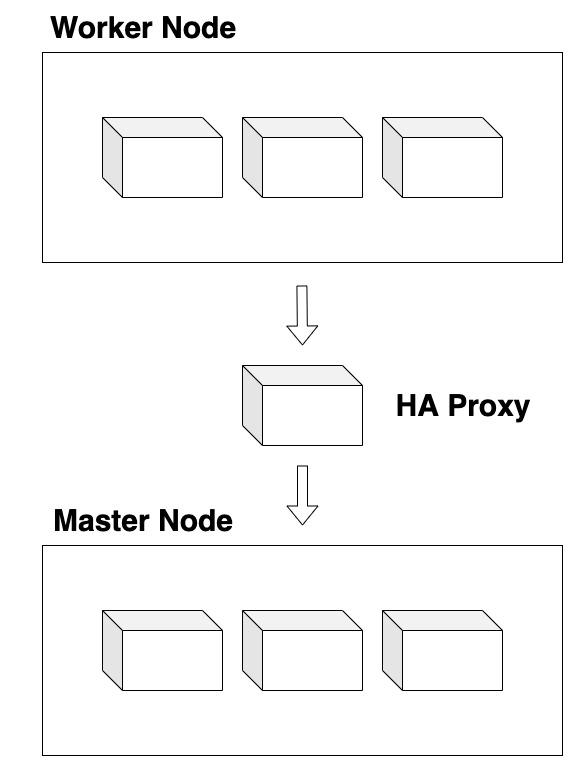
\includegraphics[width=0.4\textwidth]{./figures/haproxy.jpg}
    \caption{マスターノードとワーカーノードの関係性}
  \end{center}
\end{figure}

次に,マスターノードとワーカーノードを立ち上げるにあたり必要なパッケージをインストールした.
Kuberntesのランタイムとして使用するDockerに加え,クラスタ構築時に用いるkubeadmとkubelet, クラスタ操作時に必要なkubectlをaptによって取得した.
パッケージの用意が完了したのち,マスターノードからクラスタ構築作業を行った.
kubeadmではクラスタの初期化用にinitコマンドが用意されており,初めのマスターノードにて実行することでクラスタの基盤を作成可能である.
初期化に成功した場合,以下のようなテキストが出力される.\\

\begin{lstlisting}
  You can now join any number of control-plane nodes by copying certificate authorities
  and service account keys on each node and then running the following as root:

    kubeadm join 192.168.10.253:6443 --token { token } \
      --discovery-token-ca-cert-hash sha256:{ hash }} \
      --control-plane

  Then you can join any number of worker nodes by running the following on each as root:

  kubeadm join 192.168.10.253:6443 --token { token } \
      --discovery-token-ca-cert-hash sha256:{ hash }}
\end{lstlisting}

出力にある通り,与えられたコマンドを他のマスターノードとワーカーノードから実行することでクラスタへの参加が行える.
各サーバにて上記のコマンドを実行した結果,マスターノードからクラスタが構築できていることを確認できた.

\begin{lstlisting}
  $ kubectl get nodes
  NAME       STATUS     ROLES    AGE     VERSION
  master01   Ready      master   58d     v1.16.3
  master02   Ready      master   58d     v1.16.3
  master03   Ready      master   58d     v1.16.3
  node01     Ready      <none>   8d      v1.16.3
  node02     Ready      <none>   4d22h   v1.16.3
  node03     Ready      <none>   6d16h   v1.16.3
  node04     Ready      <none>   8d      v1.16.3
\end{lstlisting}

\section{システム全体}
\label{implementation:system}
本研究で構築した実装環境の図を以下に示す.

\begin{landscape}
  \begin{figure}[htbp]
    \begin{center}
      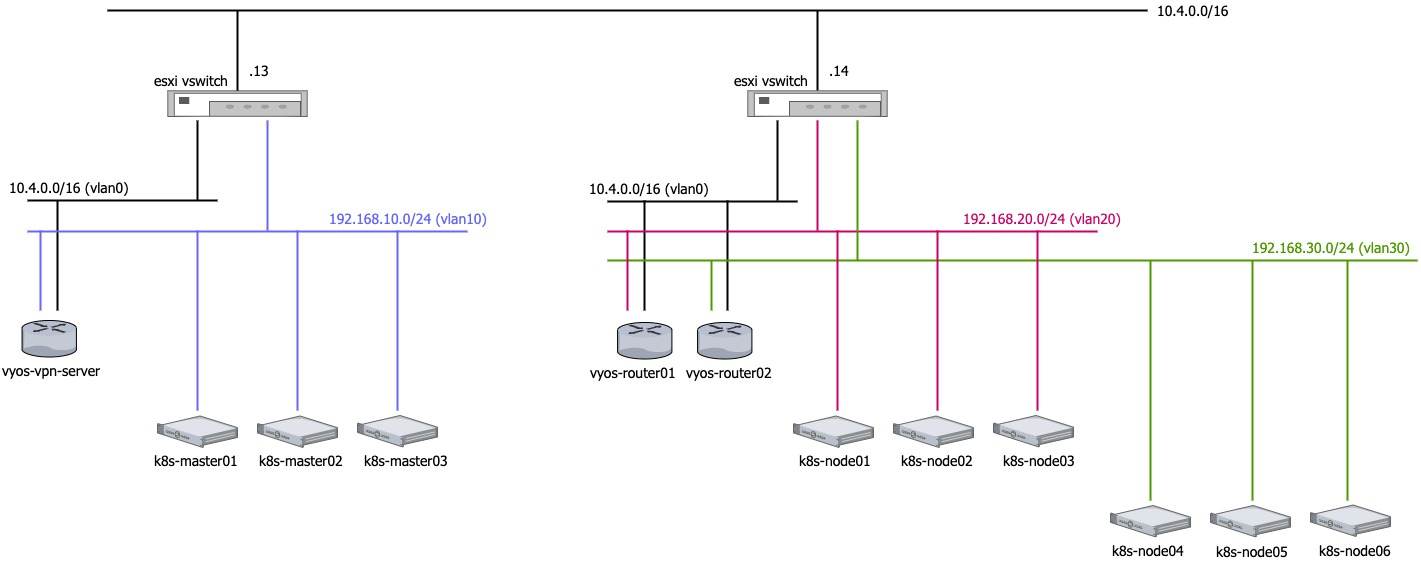
\includegraphics[width=\textwidth]{./figures/network-diagram.jpg}
      \caption{ネットワーク構成図}
    \end{center}
  \end{figure}
\end{landscape}

%%% Local Variables:
%%% mode: japanese-latex
%%% TeX-master: "../bthesis"
%%% End:

\chapter{評価}
\label{evaluation}
本章では,提案システムの評価について述べる.

\section{評価内容}



%%% Local Variables:
%%% mode: japanese-latex
%%% TeX-master: "./thesis"
%%% End:

\chapter{結論}
\label{conclusion}

本章では,本研究のまとめと今後の課題を示す.

\section{まとめ}
\label{conclusion:conclusion}

本研究では,惑星規模の分散システムの試験を行うための試験環境の構築手法を提案した.
惑星規模の分散システムは,地理的に分散したコンピュータによって構成されるため,
試験においてはネットワーク上の通信の遅延を考慮する必要があることを~\ref{background}章で示した.
~\ref{issue}章では,既存の提案手法としてPlanetLab,クラウドサービスのリージョンの活用,BSafe.networkをあげたが,
それぞれに欠点があり未だ惑星規模の分散システムの試験環境の構築手法に課題が残されていることを指摘した.
加えて,惑星規模の分散システムの試験における以下四点の必要要件を明らかにした.
\begin{itemize}
  \item OSやCPU, Memoryといったサーバ環境を柔軟に変更可能であること
  \item 公の実稼働環境を想定したネットワークでの通信の遅延を考慮できること
  \item 異なる管理権限下にある各サーバに対し統合的管理が可能であり,各オペレータの手作業を軽減できること
\end{itemize}
上記の必要要件を満たすため,本研究ではOpenVPNとKubernetesを組み合わせた惑星規模の分散システムのための構築手法を提案した.
試験環境を構成するサーバ間をOpenVPNオーバーレイネットワークによって繋げ,その上でKubernetesクラスタを構築することで,
地理的に分散したサーバを統合的に管理することができるのではないかと考えた.
~\ref{implementation}章では,提案手法の構築を行った.
ESXiを利用して仮想的にネットワーク環境を構築し,疎通性のないセグメント間でKubernetesクラスタを立ち上げた.
~\ref{evaluation}章では,~\ref{issue}章で明らかにした惑星規模の分散システムの試験環境における必要要件を本システムが満たせているか評価を行なった.
ネットワーク上の別セグメントに位置するサーバによるKubernetesクラスタが,各サーバに対し統括的な指示ができることより,
本システムが本研究の課題に対する必要要件を満たせていることを確認した.
本節の冒頭でも述べたように,惑星規模の分散システムではネットワークでの通信の遅延がシステムに影響を及ぼす.
そのため,通信の遅延を考慮した上で各コンピュータが協調動作できていることを試験しなければならず,惑星規模の分散システムのための試験環境を構築することは容易ではない.
本研究は,地理的に分散したコンピュータによって構成される分散システムの試験環境を構築手法を提案するものであり,
システムの堅牢性の向上に繋がったと考える.

\section{課題と展望}
\label{conclusion:issue}

本節では,本研究の課題と展望について述べる.
本研究の実装は,ESXiによって構築した仮想ネットワーク上で異なるセグメントを繋ぐOpenVPNオーバーレイネットワークを実装し,
さらにその上でKubernetesクラスタの構築を行なった.
実装はLAN内で行なったものであり,実際に地理的に分散したコンピュータを用いて実装が行えなかった点は課題として残された.
実用に向けた次の段階としては,本研究て提案したシステムを公のインターネット上で実装し再評価する必要があると考える.
Bitcoinの基盤技術であるブロックチェーンが登場したことによって,惑星規模の分散システムには今後より注目が集まると考える.
今後,惑星規模の分散システムの堅牢性をより一層向上させる必要があり,そのためには試験環境の提案手法の確立が大きな課題である.

%%% Local Variables:
%%% mode: japanese-latex
%%% TeX-master: "../thesis"
%%% End:

%\input{src/appendix}
\chapter{謝辞}
\addcontentsline{toc}{chapter}{謝辞}
\label{thanks}

本論文の執筆にあたり,常に優しく,最後まで見捨てずにご指導してくださった慶應義塾大学政策・メディア研究科特任准教授鈴木茂哉博士,
同大学政策・メディア研究科博士課程阿部涼介氏に感謝致します.お忙しいにも関わらず,毎週のようにミーティングを設けてくださったこと,
研究について一から教えてくださったこと,行き詰まっている際に親身に相談に乗ってくださったことには本当に感謝しております.

%%% Local Variables:
%%% mode: japanese-latex
%%% TeX-master: "../yummy_bthesis"
%%% End:


\renewcommand{\thechapter}{\Alph{chapter}}
\setcounter{chapter}{0}
\vspace{-5mm}


\input{bib/biblio}\thispagestyle{plain}%bibtex


\end{document}

%%% Local Variables:
%%% mode: japanese-latex
%%% TeX-master: t
%%% End:
